\documentclass[12pt,a4paper]{article}
\usepackage[utf8]{inputenc}
\usepackage[T1]{fontenc}
\usepackage[spanish]{babel}
\usepackage{graphicx}
\usepackage{amsmath}
\usepackage{physics}
\usepackage{geometry}
\usepackage{caption}
\usepackage{setspace}
\geometry{margin=2.5cm}
\setstretch{1.2}

\title{\textbf{Análisis físico del oscilador de Duffing acoplado}}
\author{
Eric Jesús Arciniegas Barreto \\ 
Santiago Suárez Sánchez \\ [0.5em]
\small Universidad Distrital Francisco José de Caldas
}
\date{2025}

\begin{document}
\maketitle

\section{Introducción}

El oscilador de Duffing, propuesto por Georg Duffing a comienzos del siglo XX, describe un sistema oscilatorio no lineal caracterizado por una fuerza restauradora con término cúbico. Este modelo ha sido fundamental en el desarrollo de la teoría del caos y la dinámica no lineal, pues sirve como referencia para el estudio de sistemas físicos reales que presentan oscilaciones no armónicas, tales como péndulos elásticos, circuitos RLC o estructuras vibrantes.

Debido a la riqueza de su dinámica, el oscilador de Duffing constituye un marco ideal para analizar cómo pequeñas perturbaciones pueden alterar significativamente la evolución de un sistema. Extender este estudio hacia el acoplamiento de dos osciladores resulta natural, ya que los sistemas físicos rara vez son aislados: suelen interactuar, generando comportamientos colectivos complejos.

\section{Modelo Matemático}

El sistema está compuesto por dos osciladores de Duffing idénticos, acoplados linealmente mediante un término de interacción proporcional a la diferencia de posiciones. Cada oscilador obedece la ecuación:

\begin{equation}
m\ddot{x}_1 + \gamma \dot{x}_1 + \alpha x_1 + \beta x_1^3 + k(x_1 - x_2) = G_0 \cos(\omega t),
\end{equation}
\begin{equation}
m\ddot{x}_2 + \gamma \dot{x}_2 + \alpha x_2 + \beta x_2^3 + k(x_2 - x_1) = 0.
\end{equation}

Aquí, $\alpha < 0$ determina la fuerza restauradora lineal, $\beta > 0$ la no linealidad cúbica, $\gamma$ el coeficiente de fricción, $k$ el acoplamiento entre osciladores, y $\omega$ la frecuencia de la excitación externa. Solo el primer oscilador es forzado externamente.

\section{Métodos Numéricos}

Para resolver el sistema se empleó el método de Runge–Kutta de cuarto orden (RK4), que aproxima la solución a partir de una combinación ponderada de pendientes intermedias. Este procedimiento garantiza una alta estabilidad numérica y precisión, permitiendo capturar el comportamiento no lineal del sistema durante largos intervalos de tiempo.

Las simulaciones se implementaron en \texttt{C++}, utilizando una estructura modular orientada a objetos. El programa calcula simultáneamente las trayectorias $(x_1, \dot{x}_1, x_2, \dot{x}_2)$ y permite la generación automática de los archivos de datos para graficar el espacio de fases, las secciones de Poincaré y el exponente de Lyapunov.

\section{Análisis Físico}

\subsection{Dinámica general}

El acoplamiento entre los osciladores introduce una transferencia de energía que puede alterar la periodicidad de las trayectorias. Para ciertos valores de $k$, el sistema muestra una coexistencia entre modos periódicos y cuasiperiódicos. A valores intermedios de excitación, la no linealidad cúbica y el término de acoplamiento producen una compleja interacción entre ambos osciladores, revelando regímenes caóticos caracterizados por trayectorias irregulares en el espacio de fases.

\subsection{Diagramas de espacio de fases}

\vspace{1em}
\begin{center}
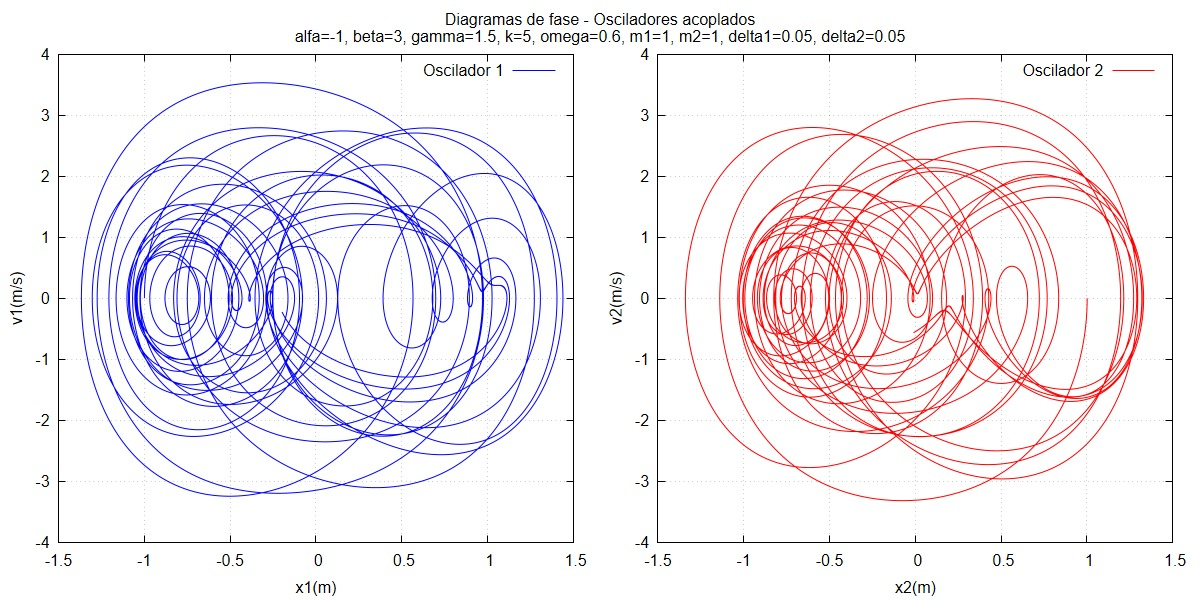
\includegraphics[width=0.8\textwidth]{figs/fase_placeholder.png}
\captionof{figure}{\textbf{Diagramas de espacio de fases.} Relación entre posición y velocidad $(x_i, \dot{x}_i)$ para cada oscilador. Las trayectorias cerradas indican comportamiento periódico, mientras que las trayectorias irregulares y dispersas corresponden a regímenes caóticos.}
\end{center}
\vspace{1em}

El análisis de los diagramas de fase permite distinguir claramente entre los diferentes regímenes dinámicos del sistema. En condiciones de baja excitación, las trayectorias forman elipses estables similares al oscilador armónico simple. A medida que se incrementa la amplitud de la fuerza externa o el acoplamiento, las trayectorias se distorsionan, apareciendo bucles y separatrices que delimitan regiones caóticas. Este tipo de representación es clave para visualizar la transición entre orden y caos.

\subsection{Secciones de Poincaré}

\vspace{1em}
\begin{center}
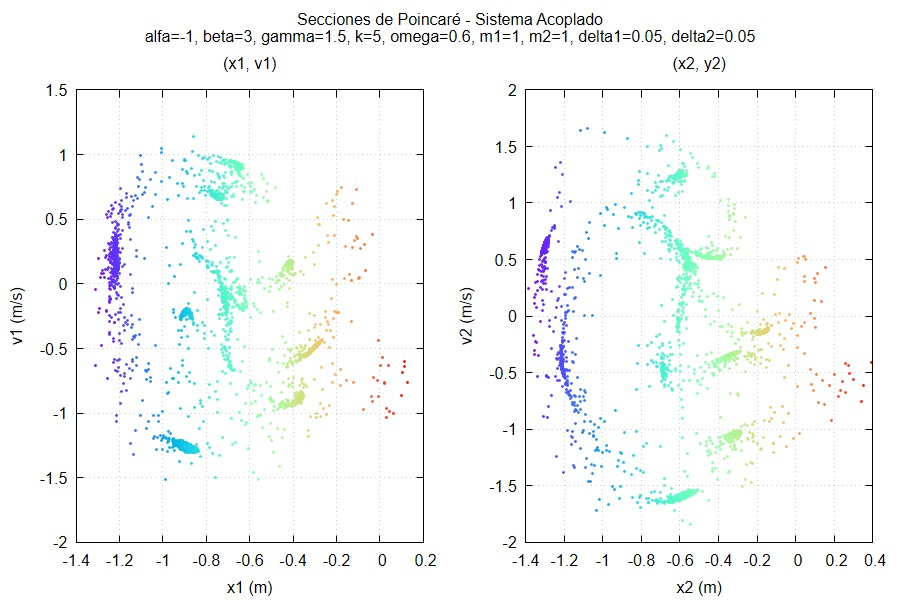
\includegraphics[width=0.8\textwidth]{figs/poincare_placeholder.png}
\captionof{figure}{\textbf{Sección de Poincaré.} Representa los puntos de intersección del sistema en cada múltiplo del periodo forzante $T = \frac{2\pi}{\omega}$.}
\end{center}
\vspace{1em}

Las secciones de Poincaré permiten visualizar la naturaleza del régimen dinámico: distribuciones discretas indican periodicidad, estructuras cerradas sugieren cuasiperiodicidad, mientras que patrones dispersos revelan un comportamiento caótico. En el caso estudiado, las figuras obtenidas muestran regiones de alta densidad de puntos mezcladas con zonas dispersas, lo que indica la coexistencia de modos cuasiperiódicos y caóticos.

\subsection{Exponente de Lyapunov}

\vspace{1em}
\begin{center}
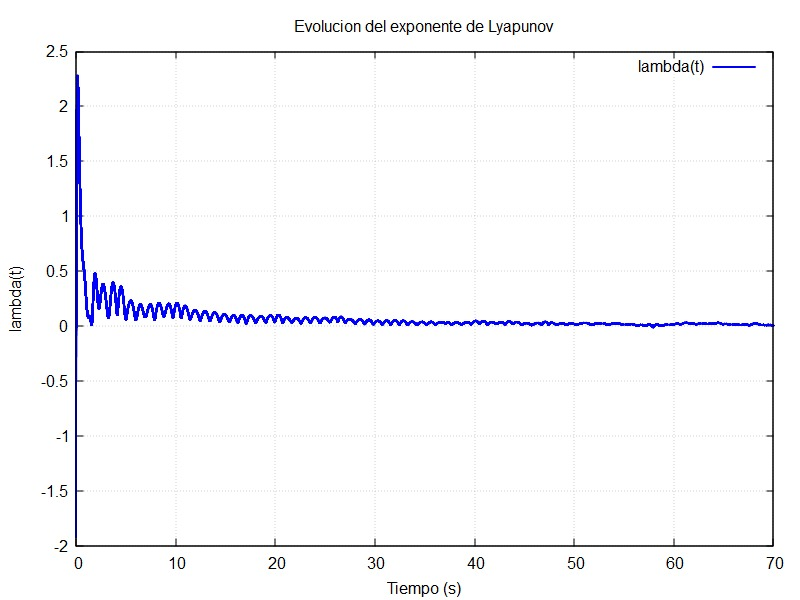
\includegraphics[width=0.8\textwidth]{figs/lyapunov_placeholder.png}
\captionof{figure}{\textbf{Evolución del exponente de Lyapunov.} Mide la sensibilidad a las condiciones iniciales y permite distinguir entre regímenes estables y caóticos.}
\end{center}
\vspace{1em}

El exponente de Lyapunov cuantifica la divergencia de trayectorias inicialmente cercanas:
\[
\lambda(t) = \frac{1}{t} \ln \left( \frac{\Delta(t)}{\Delta(0)} \right).
\]
Un valor $\lambda > 0$ indica caos determinista, mientras que $\lambda \approx 0$ sugiere cuasiperiodicidad y $\lambda < 0$ estabilidad. Los resultados muestran que el sistema mantiene un exponente positivo que tiende gradualmente a cero, lo cual refleja un caos débil o transitorio.

\section{Conclusiones}

El estudio evidencia que el acoplamiento lineal no destruye la naturaleza caótica inherente al oscilador de Duffing, sino que la modula. Bajo ciertas condiciones, los osciladores muestran sincronización parcial y regiones de cuasiperiodicidad, mientras que en otras persiste un caos controlado. Este modelo resulta un laboratorio ideal para explorar fenómenos de sincronización, bifurcaciones y transición al caos en sistemas acoplados.

\section*{Referencias}
\begin{enumerate}
    \item Scholarpedia. \textit{Duffing Oscillator}. \url{https://www.scholarpedia.org/article/Duffing_oscillator}.
    \item S. H. Strogatz, \textit{Nonlinear Dynamics and Chaos}, 2ª ed., Westview Press, 2018.
    \item D. H. Rothman, \textit{Lecture Notes 15–16: Poincaré Sections}, MIT OCW, 2022.
\end{enumerate}

\end{document}
